% ============================================================
% fig_coherent_sets.tex -- coherent vs. incoherent set under
% perturbation.  Columns are time, rows are with/without the
% perturbed ensemble.  Revealed in four steps, clockwise:
%   1 top-left      t0, two sets, unperturbed
%   2 top-right     t1, advected: one compact, one filamented
%   3 bottom-right  t1, with the perturbed ensemble
%   4 bottom-left   t0, with the perturbed ensemble
%
% Provides \coherentsetsfigure (a tikzpicture, no frame).
%
% Overlays:
%   \csoverlayson    four-step build (default)
%   \csoverlaysoff   all four panels at once
% Set before calling \coherentsetsfigure.
%
% NB: panels are written in reveal order so the dot fields stay
% pixel-identical from one overlay to the next.
%
% Include with:  \input{fig_coherent_sets}   (NOT \include)
% Requires:      \usepackage{tikz}
% ============================================================

\providecommand{\csoverlays}{1}
\providecommand{\csoverlayson}{\renewcommand{\csoverlays}{1}}
\providecommand{\csoverlaysoff}{\renewcommand{\csoverlays}{0}}

% \csstep{overlay spec}{content}
\providecommand{\csstep}[2]{%
  \ifnum\csoverlays=1 \only<#1>{#2}\else{#2}\fi}

\definecolor{dotred}{RGB}{205,15,15}
\definecolor{blobgray}{RGB}{168,168,168}

\providecommand{\panelframe}{%
  \draw[gray!55, line width=0.4pt] (0,0) rectangle (5,2.5);}

% \cluster{cx}{cy}{radius}{count}
\providecommand{\cluster}[4]{%
  \begin{scope}[shift={(#1,#2)}]
    \foreach \i in {1,...,#4}{
      \pgfmathsetmacro{\a}{360*rnd}
      \pgfmathsetmacro{\d}{#3*sqrt(rnd)}
      \fill[dotred] (\a:\d) circle (0.55pt);
    }
  \end{scope}}

% spiral radius, in cm, as a function of angle in degrees
\providecommand{\spiralr}[1]{0.601+0.000978*#1}

\providecommand{\coherentsetsfigure}{%
  % seed reset on every overlay so the dots never jitter
  \pgfmathsetseed{11}%
  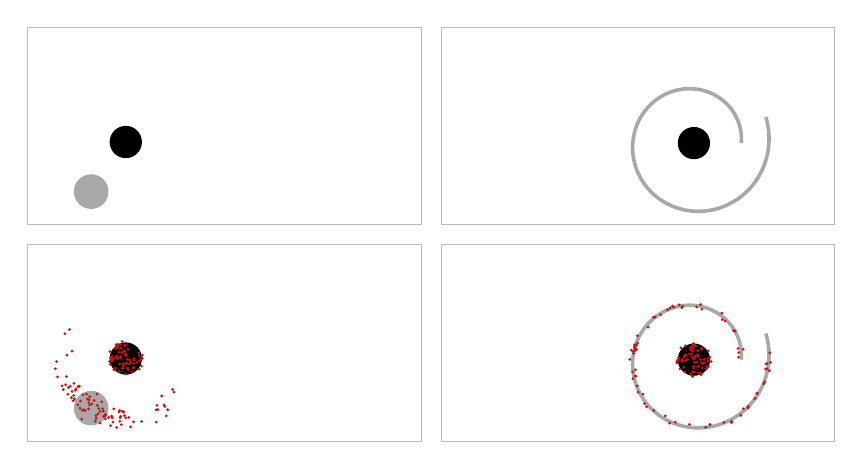
\begin{tikzpicture}
    % fixed bounding box: panels appear without shifting layout
    \path[use as bounding box] (0,0) rectangle (10.25,5.25);

    % ---------- 1: top-left -- t0, unperturbed ----------
    \csstep{4-}{%
      \begin{scope}[shift={(0,2.75)}]
        \panelframe
        \fill[black]    (1.246,1.048) circle (0.205);
        \fill[blobgray] (0.806,0.418) circle (0.220);
      \end{scope}}

    % ---------- 2: top-right -- t1, unperturbed ----------
    \csstep{5-}{%
      \begin{scope}[shift={(5.25,2.75)}]
        \panelframe
        \begin{scope}[shift={(3.211,1.034)}]
          \draw[blobgray, line width=1.3pt, smooth]
            plot[domain=0:380, samples=140, variable=\t]
            ({\t}:{\spiralr{\t}});
        \end{scope}
        \fill[black] (3.211,1.034) circle (0.205);
      \end{scope}}

    % ---------- 3: bottom-right -- t1, with ensemble ----------
    \csstep{6-}{%
      \begin{scope}[shift={(5.25,0)}]
        \panelframe
        \begin{scope}[shift={(3.211,1.034)}]
          \draw[blobgray, line width=1.3pt, smooth]
            plot[domain=0:380, samples=140, variable=\t]
            ({\t}:{\spiralr{\t}});
          \foreach \i in {1,...,72}{
            \pgfmathsetmacro{\t}{380*rnd}
            \pgfmathsetmacro{\r}{\spiralr{\t}+0.038*rand}
            \fill[dotred] ({\t}:{\r}) circle (0.55pt);
          }
        \end{scope}
        \fill[black] (3.211,1.034) circle (0.205);
        \cluster{3.211}{1.034}{0.225}{70}
      \end{scope}}

    % ---------- 4: bottom-left -- t0, with ensemble ----------
    \csstep{7-}{%
      \begin{scope}[shift={(0,0)}]
        \panelframe
        \fill[black]    (1.246,1.048) circle (0.205);
        \fill[blobgray] (0.806,0.418) circle (0.220);
        % coherent set: ensemble stays on the blob
        \cluster{1.246}{1.048}{0.225}{70}
        % incoherent set: ensemble strung out along the emerging
        % filament -- an arc about the coherent set, the first
        % part of the spiral fully wound in the top-right panel
        \begin{scope}[shift={(1.246,1.048)}]
          \foreach \i in {1,...,45}{
            \pgfmathsetmacro{\t}{205+70*rnd}
            \pgfmathsetmacro{\r}{0.777+0.115*rand}
            \fill[dotred] (\t:\r) circle (0.55pt);
          }
          \foreach \i in {1,...,33}{
            \pgfmathsetmacro{\t}{150+180*rnd}
            \pgfmathsetmacro{\r}{0.777+0.130*rand}
            \fill[dotred] (\t:\r) circle (0.55pt);
          }
        \end{scope}
        \cluster{0.806}{0.418}{0.20}{12}
      \end{scope}}
  \end{tikzpicture}}